\documentclass[10pt,twocolumn]{article}
\usepackage[top=0.9in,bottom=0.9in,left=0.75in,right=0.75in,columnsep=0.3in]{geometry}
\usepackage{graphicx,amsmath,amssymb,booktabs,cite,times}
\setlength{\parindent}{1em}\linespread{1.1}
\begin{document}
\title{\vspace{-1em}\large\bfseries Reproducing Mamba at Small Scale: Selective State Spaces versus Time-Invariant SSMs and Transformers\vspace{-0.5em}}
\author{\small Deep Learning 2026 --- Paper Implementation Project (DL-061)\\ \small [Your name, roll number]}
\date{}
\maketitle\vspace{-1.5em}

\begin{abstract}
\small We re-implement the selective state-space (S6) block of Mamba \cite{gu2023mamba} in pure PyTorch and test its central claim at small scale on a Colab T4 GPU. On a synthetic selective-copying task, the selective model reaches 82.2\% sequence accuracy while an otherwise identical input-independent (LTI) model reaches 0\%; a parameter-matched Transformer reaches 100\% at this short sequence length. On a TinyShakespeare character-level language model (about 475K parameters), the selective and LTI models are indistinguishable (2.383 vs.\ 2.385 bits/char), and both beat the parameter-matched Transformer (2.514). All results are from a single seed. We therefore claim only that selection is necessary for selective copying in our setting, and that we could not show a benefit of selection on language modeling at this scale.
\end{abstract}

\section{Problem and Motivation}
Transformers model sequences with $O(L^2)$ attention. Linear-time alternatives based on structured state-space models (SSMs) such as S4 \cite{s4} are linear time-invariant (LTI): the same dynamics apply at every position, so they cannot decide what to remember based on content. Mamba makes the SSM parameters functions of the input and recovers efficiency with a hardware-aware scan. We ask: (i) does selectivity matter on a task designed to need it; (ii) does it help on language modeling at small scale; (iii) how does Mamba compare with a Transformer of equal parameter count?

\section{Background and Method}
A continuous SSM $h'(t)=Ah(t)+Bx(t),\ y(t)=Ch(t)$ is discretised with step size $\Delta$. Assuming $x$ is constant over each step (zero-order hold), the exact solution gives
\begin{equation}
\bar A=e^{\Delta A},\qquad \bar B=(\Delta A)^{-1}\!\left(e^{\Delta A}-I\right)\Delta B\approx\Delta B,
\end{equation}
where the approximation is the Euler form used in practice (accurate for small $\Delta$). The recurrence is
\begin{equation}
h_t=\bar A_t h_{t-1}+\bar B_t x_t,\qquad y_t=C_t h_t+Dx_t .
\end{equation}
With $A$ diagonal and negative, $\bar A\in(0,1)$ element-wise, so the state decays and the update is stable. In an LTI model $(\Delta,B,C)$ are constants, so the model equals a global convolution. In S6 they are \emph{selective}: $\Delta_t=\mathrm{softplus}(\mathrm{Lin}(x_t))$, $B_t=\mathrm{Lin}_B(x_t)$, $C_t=\mathrm{Lin}_C(x_t)$. Intuitively, $B_t$ decides what to write, $C_t$ what to read, and $\Delta_t$ how strongly the current input replaces the state (large $\Delta$: reset to the current input; small $\Delta$: ignore it). Selectivity breaks the convolutional view, but the recurrence stays associative under
\begin{equation}
(a_1,b_1)\circ(a_2,b_2)=(a_1a_2,\;a_2b_1+b_2),
\label{eq:assoc}
\end{equation}
so it can be computed by a parallel prefix scan. Costs: attention is $O(L^2D)$ in time; the SSM is $O(LDN)$ in time with $O(DN)$ state at inference.


\subsection{Derivation of the discretisation}
For $h'=Ah+Bx$ with $x$ held constant over $[t,t{+}\Delta]$, the variation-of-constants formula gives
\begin{equation}
h(t{+}\Delta)=e^{\Delta A}h(t)+\int_0^{\Delta}e^{(\Delta-s)A}B\,ds\;x
=e^{\Delta A}h(t)+A^{-1}\!\left(e^{\Delta A}-I\right)B\,x .
\end{equation}
Hence $\bar A=e^{\Delta A}$ and $\bar B=A^{-1}(e^{\Delta A}-I)B=(\Delta A)^{-1}(e^{\Delta A}-I)\,\Delta B$. For small $\Delta A$, $(\Delta A)^{-1}(e^{\Delta A}-I)\to I$, so $\bar B\approx\Delta B$. The notebook compares the two for $A=-(1,2,3)$: at $\Delta{=}0.01$ they agree to within 1\%, at $\Delta{=}0.1$ they differ by about 5--14\%, and at $\Delta{=}1$ they differ substantially ($\bar B=0.63$ vs.\ $1.0$ for the first state dimension). Since $\Delta$ is initialised in $[10^{-3},10^{-1}]$ and learned, we use the cheaper Euler form as the paper does.

\subsection{Why the recurrence is parallelisable}
Write the update as an affine map $h\mapsto a\,h+b$. Composing two such maps gives $h\mapsto a_2(a_1h+b_1)+b_2=(a_1a_2)h+(a_2b_1+b_2)$, which is Eq.~\eqref{eq:assoc}. Because this composition is associative, all prefixes $h_1,\dots,h_L$ can be computed by a parallel scan with depth $O(\log L)$ instead of $L$ sequential steps. Selectivity makes $a_t=\bar A_t$ and $b_t=\bar B_tx_t$ depend on the input, but they are still known for all $t$ before the scan starts, so associativity is all that is needed.
\section{Implementation}
All code was written for this project in PyTorch (notebook \texttt{Mamba\_from\_scratch.ipynb}). \textbf{Block:} \texttt{in\_proj} produces $(x,z)$ of width $2D_{\text{in}}$ (expand 2); $x$ passes through a causal depthwise convolution (kernel 4, left padding $k{-}1$, cropped to length $L$) and SiLU; $(\Delta,B,C)$ come from \texttt{x\_proj} and \texttt{dt\_proj} (low-rank, rank $\lceil d/16\rceil$); the scan output is gated by $\mathrm{SiLU}(z)$ and projected by \texttt{out\_proj}. $A=-\exp(A_{\log})$ is initialised S4D-real ($A=-(1,\dots,N)$) and $\Delta$ such that $\mathrm{softplus}(\text{bias})$ is log-uniform in $[10^{-3},10^{-1}]$, as in the paper.

\textbf{Scan:} we implement a sequential reference scan (Python loop) and a Hillis--Steele parallel scan using Eq.~\eqref{eq:assoc}: in round $k$ every position combines with the one $2^k$ steps earlier, so $h_{1:L}$ is obtained in $\lceil\log_2L\rceil$ rounds. The parallel scan materialises tensors of shape $(B,L,D_{\text{in}},N)$, so it is far less memory-efficient than the paper's fused CUDA kernel. Two unit tests are in the notebook: the two scans agree (max abs.\ difference $9.5{\times}10^{-7}$), and the block is causal (perturbing inputs at positions $\ge10$ leaves outputs before position 10 unchanged).


\begin{figure}[h]\small\centering\fbox{\parbox{0.94\columnwidth}{\textbf{Algorithm 1: selective scan} (batch $b$, length $l$, channels $d$, state $n$).\\
\textbf{Input:} $u,\Delta\in\mathbb R^{b\times l\times d}$, $A\in\mathbb R^{d\times n}$, $B,C\in\mathbb R^{b\times l\times n}$, $D\in\mathbb R^{d}$\\
1. $\bar A\leftarrow\exp(\Delta\otimes A)$ \hfill $(b,l,d,n)$\\
2. $\bar Bu\leftarrow\Delta\otimes B\otimes u$ \hfill $(b,l,d,n)$\\
3. \emph{sequential:} for $t=1..l$: $h\leftarrow\bar A_t\odot h+\bar Bu_t$;\ $y_t\leftarrow\sum_n C_{t,n}h_{\cdot,n}$\\
\hspace{0.9em}\emph{parallel:} for $o=1,2,4,\dots<l$: $\;x_t\leftarrow\bar A_t\odot x_{t-o}+x_t$,\ $\bar A_t\leftarrow\bar A_t\odot\bar A_{t-o}$ (positions $t\le o$ unchanged); then $y_t\leftarrow\sum_nC_{t,n}x_{t,\cdot,n}$\\
4. \textbf{return} $y+D\odot u$}}\label{alg:scan}\end{figure}
\textbf{Design choices.} Weight decay is applied to all parameters for simplicity (the official code exempts $A_{\log}$ and $D$), a small deviation from the reference implementation. We use RMSNorm before each mixer, residual connections, and tie the embedding and output head. The Transformer baseline uses learned absolute positions of the same width as the model; its attention uses a boolean causal mask. Data for both tasks is generated on the fly from fixed seeds, and evaluation uses a fixed held-out generator (selective copy: 512 fresh sequences; LM: 20 validation batches).
\textbf{Models.} Both architectures share one wrapper: embedding, $n$ layers of (RMSNorm $\to$ mixer $\to$ residual), final RMSNorm, and a weight-tied output head. The mixer is either the Mamba block or a causal pre-norm Transformer block (4 heads, GELU MLP, learned absolute positions). \textbf{LTI ablation:} $\Delta$, $B$, $C$ are replaced by input-independent learned parameters ($\Delta$ per channel, $B,C\in\mathbb R^N$ shared), with the same initialisation of $\Delta$ and $A$; all else is unchanged.

\textbf{Equal size.} ``Equal size'' means equal total parameter count. The Transformer has the same width and depth as Mamba, and its MLP width $d_{\text{ff}}$ is chosen so that its total parameters match the selective Mamba model (parameters are linear in $d_{\text{ff}}$): $d_{\text{ff}}=105$ for copying and $179$ for the LM. The LTI ablation is \emph{not} size-matched: it has about 15\% (copy) and 10\% (LM) fewer parameters because it has no \texttt{x\_proj}.

\section{Experimental Setup}
\textbf{Tasks.} \emph{Selective copying}: $K{=}8$ data tokens (vocabulary 8) are placed at random positions among noise tokens (token 0) in a window of $L{=}64$, followed by $K$ recall markers; the target at the marker positions is the data tokens in order. Loss and accuracy are measured on those $K$ positions; \emph{sequence accuracy} requires all $K$ correct, \emph{token accuracy} is per token (chance level is $1/8$). \emph{Character LM}: TinyShakespeare (1.12M characters, vocabulary 65), 90/10 train/validation split, context 128; the metric is validation bits per character (cross-entropy in nats divided by $\ln2$).

\textbf{Changes from the paper.} The paper evaluates selective copying at $L{=}4096$ with 16 tokens and trains much larger language models on large corpora. We use $L{=}64$, $K{=}8$, two-layer models, and a 475K-parameter LM trained for 4000 steps, so that everything runs on a free T4. Absolute numbers are not comparable to the paper; only qualitative comparisons are meaningful.

\begin{table}[h]\centering\small\caption{Training configuration (Colab T4, single run, seed 0).}
\begin{tabular}{lcc}\toprule
 & Selective copy & Char LM\\\midrule
$d_{\text{model}}$ / layers / $N$ & 64 / 2 / 16 & 128 / 4 / 16\\
Context & 64+8 & 128\\
Batch / steps & 64 / 3000 & 32 / 4000\\
Peak lr & $3{\times}10^{-3}$ & $2{\times}10^{-3}$\\
Optimizer & \multicolumn{2}{c}{AdamW, wd 0.01, one-cycle (10\% warmup), clip 1.0}\\\bottomrule
\end{tabular}\end{table}

\section{Results}
\begin{table}[h]\centering\small\caption{Selective copying after 3000 steps ($K{=}8$, $L{=}64$).}
\begin{tabular}{lcccc}\toprule
Model & Params & Tok.\ acc. & Seq.\ acc. & Time\\\midrule
Mamba & 66.1K & 0.976 & 0.822 & 325 s\\
Mamba-LTI & 55.9K & 0.504 & 0.000 & 325 s\\
Transformer & 66.1K & 1.000 & 1.000 & 26 s\\\bottomrule
\end{tabular}\end{table}
\begin{figure*}[t]\centering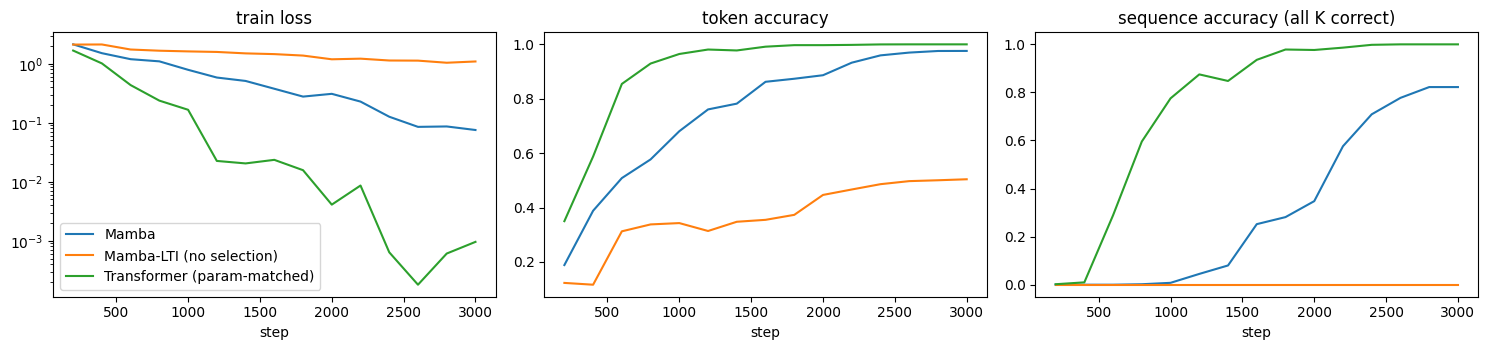
\includegraphics[width=0.92\textwidth]{copy_curves.png}\caption{Selective copying ($L{=}64$, $K{=}8$): training loss (log scale), token accuracy and sequence accuracy for the three models.}\end{figure*}

\begin{table}[h]\centering\small\caption{TinyShakespeare after 4000 steps (validation).}
\begin{tabular}{lcccc}\toprule
Model & Params & Bits/char & Perplexity & Time\\\midrule
Mamba & 474.9K & 2.383 & 5.22 & 1585 s\\
Mamba-LTI & 425.9K & 2.385 & 5.22 & 1577 s\\
Transformer & 474.6K & 2.514 & 5.71 & 64 s\\\bottomrule
\end{tabular}\end{table}
\begin{figure}[h]\centering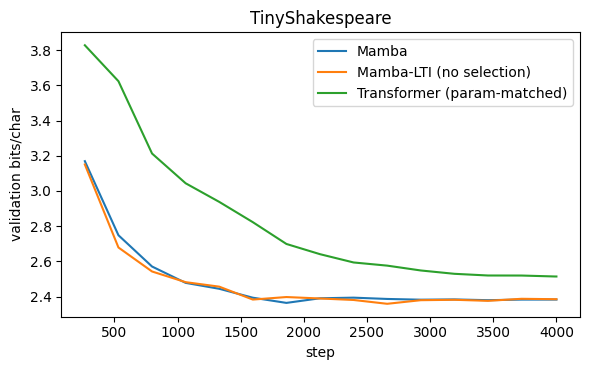
\includegraphics[width=0.85\columnwidth]{lm_curves.png}\caption{Validation bits/char on TinyShakespeare (lower is better).}\end{figure}

\textbf{Selective copying.} Selection is clearly necessary: the LTI model never reproduces a full sequence (0.0\%) and plateaus around 50\% token accuracy, while the selective model reaches 82.2\%. (The LTI model's partial token accuracy is well above chance, $12.5\%$; we did not investigate what it exploits.) The Transformer, however, solves the task completely, reaching 100\% sequence accuracy by about step 2600, much faster than Mamba. Mamba's sequence accuracy rose from 0.58 at step 2200 to 0.78 at step 2600 and then flattened near 0.82 as the one-cycle learning rate decayed to zero; we do not know whether a longer schedule would close the gap to the Transformer.

\textbf{Language modeling.} The selective and LTI Mamba models are indistinguishable (2.383 vs.\ 2.385 bits/char, perplexity 5.22 for both; the curves cross repeatedly), so we cannot claim that selectivity helps here. Both Mamba variants are about 0.13 bits/char better than the parameter-matched Transformer (2.514), whose validation loss was still decreasing slowly at the end of training. Wall-clock times (Mamba about 12$\times$ slower than the Transformer on copying and 25$\times$ on the LM) reflect our Python-level parallel scan, not the paper's fused kernel, and should not be read as a property of the architectures.

\section{Ablation}
The ablation removes input dependence of $\Delta$, $B$ and $C$ simultaneously. On selective copying this reduces sequence accuracy from 82.2\% to 0\% and token accuracy from 97.6\% to 50.4\%, consistent with the paper's argument: a time-invariant system applies the same dynamics at every position and cannot choose which tokens to keep. On the LM the same ablation changes bits/char by 0.002, i.e.\ no measurable effect. Caveats: the LTI model has fewer parameters, so the comparison is not size-matched (though a $\sim$15\% difference seems unlikely to explain a gap from 82\% to 0\%); and we did not ablate $\Delta$, $B$ and $C$ separately, which the paper does (finding selective $\Delta$ most important).

\section{Failure Cases and Caveats}
(i) \emph{Single seed.} All numbers come from one run, so we have no estimate of run-to-run variance; differences such as 0.13 bits/char between Mamba and the Transformer should be treated as tentative. (ii) \emph{Transformer wins at short length.} At $L{=}64$ attention can retrieve content directly and solves selective copying faster and more completely than Mamba; the paper's argument concerns much longer sequences, which we did not test. (iii) \emph{Mamba not converged on copying.} Its accuracy was still improving until the learning rate annealed, so the reported 82.2\% is likely not its ceiling; we did not test longer training. (iv) \emph{Likely overfitting on the LM.} Mamba's validation loss reached 2.364 bits/char at step 1862, was 2.394 at step 2394, and ended at 2.383; the final single-batch training loss was about 1.2--1.3 nats (about 1.8 bits/char), well below validation. Together with the 16 passes over a 1 MB corpus (4000 steps $\times$ 32 $\times$ 128 characters) this suggests overfitting, but we did not test it, e.g.\ with dropout or early stopping. (v) \emph{Not size-matched LTI.} See above. (vi) \emph{Speed.} The scan is pure PyTorch, so no efficiency claims can be made.

\section{Related Work}
S4 \cite{s4} introduced stable parameterisations of LTI SSMs for long sequences. Mamba \cite{gu2023mamba} adds input-dependent parameters and a hardware-aware scan and reports competitive language modeling with linear scaling in length. The selective-copying task follows the paper's synthetic benchmark. Our work is a small-scale re-implementation and ablation, not a new result.

\section{Conclusion}
At small scale, input-dependent selection is necessary for selective copying (82\% vs.\ 0\% sequence accuracy against an LTI ablation) but a parameter-matched Transformer still solves the task better at $L{=}64$. On TinyShakespeare, selection made no measurable difference, while both Mamba variants outperformed the matched Transformer by about 0.13 bits/char. Next steps are multiple seeds, longer sequences, separate ablations of $\Delta$, $B$ and $C$, and regularisation for the LM.

\begin{thebibliography}{9}\small
\bibitem{gu2023mamba} A. Gu and T. Dao, ``Mamba: Linear-time sequence modeling with selective state spaces,'' \emph{COLM}, 2024, arXiv:2312.00752.
\bibitem{s4} A. Gu, K. Goel, and C. R\'e, ``Efficiently modeling long sequences with structured state spaces,'' \emph{ICLR}, 2022.
\end{thebibliography}
\end{document}
